\documentclass[border=8pt]{standalone}
\usepackage[utf8]{inputenc}
\usepackage[T1]{fontenc}
\usepackage{tikz}
\usetikzlibrary{arrows.meta, positioning, shapes.geometric, fit, calc, backgrounds}

\definecolor{borderDark}{HTML}{2B2B2B}
\definecolor{appFill}{HTML}{F5F5F5}
\definecolor{obsFill}{HTML}{E6ECF2}
\definecolor{obsBorder}{HTML}{2F4858}
\definecolor{loadFill}{HTML}{EFECE6}
\definecolor{loadBorder}{HTML}{5A4E3C}
\definecolor{volFill}{HTML}{F7F7F7}
\definecolor{volBorder}{HTML}{4A4A4A}
\definecolor{netBg}{HTML}{FAFAFA}

\begin{document}
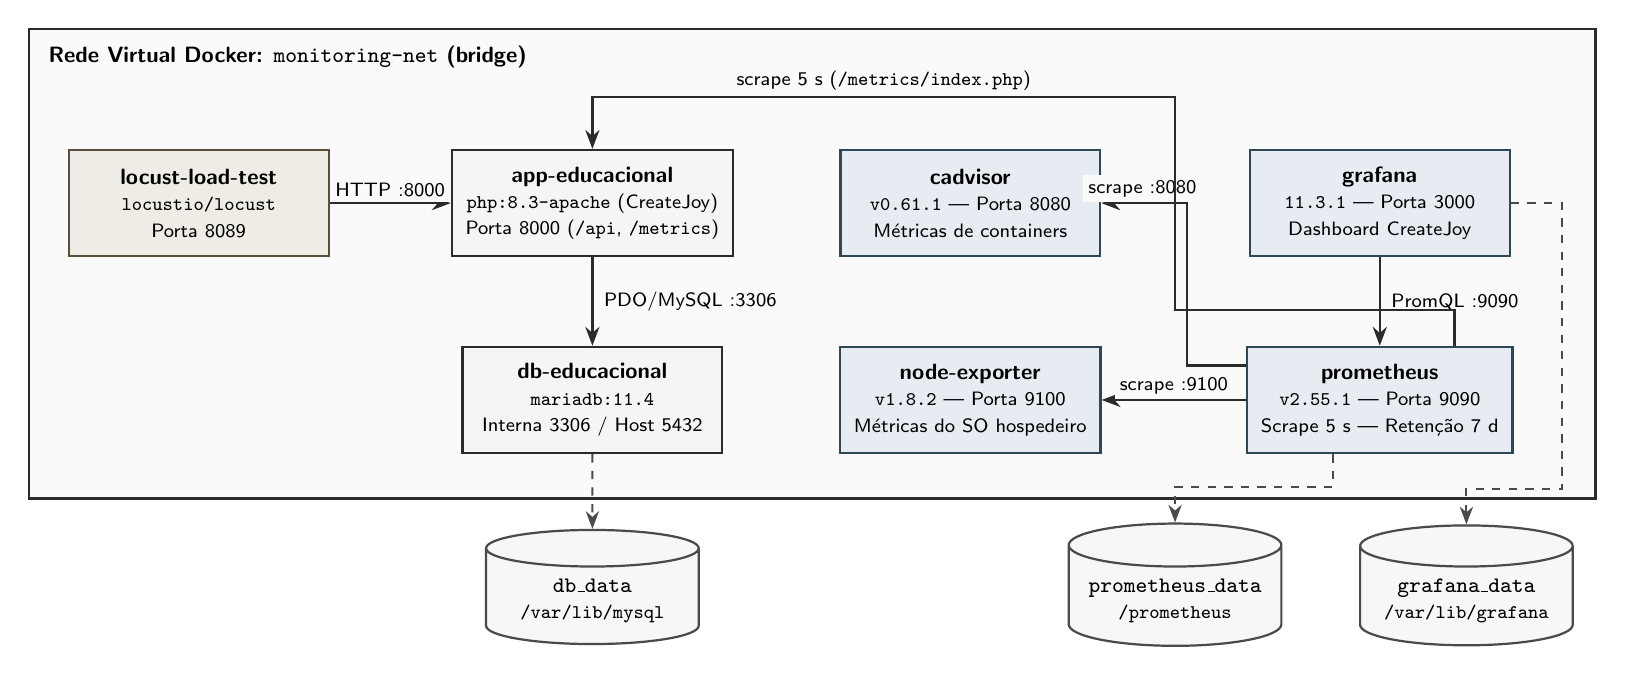
\begin{tikzpicture}[
    font=\sffamily\footnotesize,
    >=Stealth,
    box/.style={
        rectangle,
        draw=borderDark,
        line width=0.8pt,
        fill=appFill,
        minimum width=3.3cm,
        minimum height=1.35cm,
        align=center,
        inner sep=5pt
    },
    obsbox/.style={
        box,
        draw=obsBorder,
        fill=obsFill
    },
    loadbox/.style={
        box,
        draw=loadBorder,
        fill=loadFill
    },
    vol/.style={
        cylinder,
        shape border rotate=90,
        aspect=0.22,
        draw=volBorder,
        line width=0.8pt,
        fill=volFill,
        minimum width=2.7cm,
        minimum height=0.95cm,
        align=center,
        inner sep=4pt
    },
    flow/.style={
        ->,
        line width=0.85pt,
        draw=borderDark
    },
    vollink/.style={
        ->,
        dashed,
        line width=0.75pt,
        draw=volBorder
    },
    lbl/.style={
        font=\sffamily\scriptsize,
        fill=netBg,
        inner sep=1.8pt
    }
]

% Coluna 1: Carga
\node[loadbox] (locust) at (0, 2.5) {
    \textbf{locust-load-test}\\
    \scriptsize\texttt{locustio/locust}\\
    \scriptsize Porta 8089
};

% Coluna 2: Sistema Alvo
\node[box] (app) at (5.0, 2.5) {
    \textbf{app-educacional}\\
    \scriptsize\texttt{php:8.3-apache} (CreateJoy)\\
    \scriptsize Porta 8000 (\texttt{/api}, \texttt{/metrics})
};

\node[box] (db) at (5.0, 0) {
    \textbf{db-educacional}\\
    \scriptsize\texttt{mariadb:11.4}\\
    \scriptsize Interna 3306 / Host 5432
};

% Coluna 3: Coletores
\node[obsbox] (cadvisor) at (9.8, 2.5) {
    \textbf{cadvisor}\\
    \scriptsize\texttt{v0.61.1} | Porta 8080\\
    \scriptsize Métricas de containers
};

\node[obsbox] (nodeexp) at (9.8, 0) {
    \textbf{node-exporter}\\
    \scriptsize\texttt{v1.8.2} | Porta 9100\\
    \scriptsize Métricas do SO hospedeiro
};

% Coluna 4: Prometheus e Grafana
\node[obsbox] (grafana) at (15.0, 2.5) {
    \textbf{grafana}\\
    \scriptsize\texttt{11.3.1} | Porta 3000\\
    \scriptsize Dashboard CreateJoy
};

\node[obsbox] (prom) at (15.0, 0) {
    \textbf{prometheus}\\
    \scriptsize\texttt{v2.55.1} | Porta 9090\\
    \scriptsize Scrape 5 s | Retenção 7 d
};

% Ponto auxiliar superior para garantir folga para a rota superior dentro da rede
\coordinate (topguide) at (9.8, 4.15);
\coordinate (rightguide) at (17.25, 0);

% Caixa da rede Docker (atras dos nos)
\begin{scope}[on background layer]
    \node[
        draw=borderDark,
        line width=0.9pt,
        fill=netBg,
        inner xsep=14pt,
        inner ysep=16pt,
        fit=(locust) (app) (db) (cadvisor) (nodeexp) (grafana) (prom) (topguide) (rightguide),
        label={[anchor=north west, font=\sffamily\footnotesize\bfseries, xshift=4pt, yshift=-3pt]north west:Rede Virtual Docker: \texttt{monitoring-net} (bridge)}
    ] (netbox) {};
\end{scope}

% Volumes persistentes abaixo da rede
\node[vol] (voldb) at (5.0, -2.55) {
    \textbf{\texttt{db\_data}}\\
    \scriptsize\texttt{/var/lib/mysql}
};

\node[vol] (volprom) at (12.4, -2.55) {
    \textbf{\texttt{prometheus\_data}}\\
    \scriptsize\texttt{/prometheus}
};

\node[vol] (volgraf) at (16.1, -2.55) {
    \textbf{\texttt{grafana\_data}}\\
    \scriptsize\texttt{/var/lib/grafana}
};

% Fluxos de comunicacao
\draw[flow] (locust.east) -- node[above, lbl] {HTTP :8000} (app.west);
\draw[flow] (app.south) -- node[right, lbl, xshift=2pt] {PDO/MySQL :3306} (db.north);

\draw[flow] (grafana.south) -- node[right, lbl, xshift=2pt] {PromQL :9090} (prom.north);
\draw[flow] (prom.west) -- node[above, lbl] {scrape :9100} (nodeexp.east);
\draw[flow] ($(prom.north west)+(0,-0.25)$) -- ++(-0.75,0) |- node[pos=0.76, above, lbl] {scrape :8080} (cadvisor.east);

% Scrape de /metrics da aplicacao por cima sem cruzar caixas
\draw[flow] ($(prom.north)+(0.95,0)$) -- ++(0,0.45) -| (12.4, 3.85) -- node[above, lbl] {scrape 5 s (\texttt{/metrics/index.php})} (5.0, 3.85) -- (app.north);

% Ligacoes com volumes persistentes
\draw[vollink] (db.south) -- (voldb.north);
\draw[vollink] ($(prom.south)+(-0.6,0)$) |- ($(volprom.north)+(0,0.45)$) -- (volprom.north);
\draw[vollink] (grafana.east) -- ++(0.65,0) |- ($(volgraf.north)+(0,0.45)$) -- (volgraf.north);

\end{tikzpicture}
\end{document}
